\documentclass[1p]{elsarticle_modified}
%\bibliographystyle{elsarticle-num}

%\usepackage[colorlinks]{hyperref}
%\usepackage{abbrmath_seonhwa} %\Abb, \Ascr, \Acal ,\Abf, \Afrak
\usepackage{amsfonts}
\usepackage{amssymb}
\usepackage{amsmath}
\usepackage{amsthm}
\usepackage{scalefnt}
\usepackage{amsbsy}
\usepackage{kotex}
\usepackage{caption}
\usepackage{subfig}
\usepackage{color}
\usepackage{graphicx}
\usepackage{xcolor} %% white, black, red, green, blue, cyan, magenta, yellow
\usepackage{float}
\usepackage{setspace}
\usepackage{hyperref}

\usepackage{tikz}
\usetikzlibrary{arrows}

\usepackage{multirow}
\usepackage{array} % fixed length table
\usepackage{hhline}

%%%%%%%%%%%%%%%%%%%%%
\makeatletter
\renewcommand*\env@matrix[1][\arraystretch]{%
	\edef\arraystretch{#1}%
	\hskip -\arraycolsep
	\let\@ifnextchar\new@ifnextchar
	\array{*\c@MaxMatrixCols c}}
\makeatother %https://tex.stackexchange.com/questions/14071/how-can-i-increase-the-line-spacing-in-a-matrix
%%%%%%%%%%%%%%%

\usepackage[normalem]{ulem}

\newcommand{\msout}[1]{\ifmmode\text{\sout{\ensuremath{#1}}}\else\sout{#1}\fi}
%SOURCE: \msout is \stkout macro in https://tex.stackexchange.com/questions/20609/strikeout-in-math-mode

\newcommand{\cancel}[1]{
	\ifmmode
	{\color{red}\msout{#1}}
	\else
	{\color{red}\sout{#1}}
	\fi
}

\newcommand{\add}[1]{
	{\color{blue}\uwave{#1}}
}

\newcommand{\replace}[2]{
	\ifmmode
	{\color{red}\msout{#1}}{\color{blue}\uwave{#2}}
	\else
	{\color{red}\sout{#1}}{\color{blue}\uwave{#2}}
	\fi
}

\newcommand{\Sol}{\mathcal{S}} %segment
\newcommand{\D}{D} %diagram
\newcommand{\A}{\mathcal{A}} %arc


%%%%%%%%%%%%%%%%%%%%%%%%%%%%%5 test

\def\sl{\operatorname{\textup{SL}}(2,\Cbb)}
\def\psl{\operatorname{\textup{PSL}}(2,\Cbb)}
\def\quan{\mkern 1mu \triangleright \mkern 1mu}

\theoremstyle{definition}
\newtheorem{thm}{Theorem}[section]
\newtheorem{prop}[thm]{Proposition}
\newtheorem{lem}[thm]{Lemma}
\newtheorem{ques}[thm]{Question}
\newtheorem{cor}[thm]{Corollary}
\newtheorem{defn}[thm]{Definition}
\newtheorem{exam}[thm]{Example}
\newtheorem{rmk}[thm]{Remark}
\newtheorem{alg}[thm]{Algorithm}

\newcommand{\I}{\sqrt{-1}}
\begin{document}

%\begin{frontmatter}
%
%\title{Boundary parabolic representations of knots up to 8 crossings}
%
%%% Group authors per affiliation:
%\author{Yunhi Cho} 
%\address{Department of Mathematics, University of Seoul, Seoul, Korea}
%\ead{yhcho@uos.ac.kr}
%
%
%\author{Seonhwa Kim} %\fnref{s_kim}}
%\address{Center for Geometry and Physics, Institute for Basic Science, Pohang, 37673, Korea}
%\ead{ryeona17@ibs.re.kr}
%
%\author{Hyuk Kim}
%\address{Department of Mathematical Sciences, Seoul National University, Seoul 08826, Korea}
%\ead{hyukkim@snu.ac.kr}
%
%\author{Seokbeom Yoon}
%\address{Department of Mathematical Sciences, Seoul National University, Seoul, 08826,  Korea}
%\ead{sbyoon15@snu.ac.kr}
%
%\begin{abstract}
%We find all boundary parabolic representation of knots up to 8 crossings.
%
%\end{abstract}
%\begin{keyword}
%    \MSC[2010] 57M25 
%\end{keyword}
%
%\end{frontmatter}

%\linenumbers
%\tableofcontents
%
\newcommand\colored[1]{\textcolor{white}{\rule[-0.35ex]{0.8em}{1.4ex}}\kern-0.8em\color{red} #1}%
%\newcommand\colored[1]{\textcolor{white}{ #1}\kern-2.17ex	\textcolor{white}{ #1}\kern-1.81ex	\textcolor{white}{ #1}\kern-2.15ex\color{red}#1	}

{\Large $\underline{12n_{0025}~(K12n_{0025})}$}

\setlength{\tabcolsep}{10pt}
\renewcommand{\arraystretch}{1.6}
\vspace{1cm}\begin{tabular}{m{100pt}>{\centering\arraybackslash}m{274pt}}
\multirow{5}{120pt}{
	\centering
	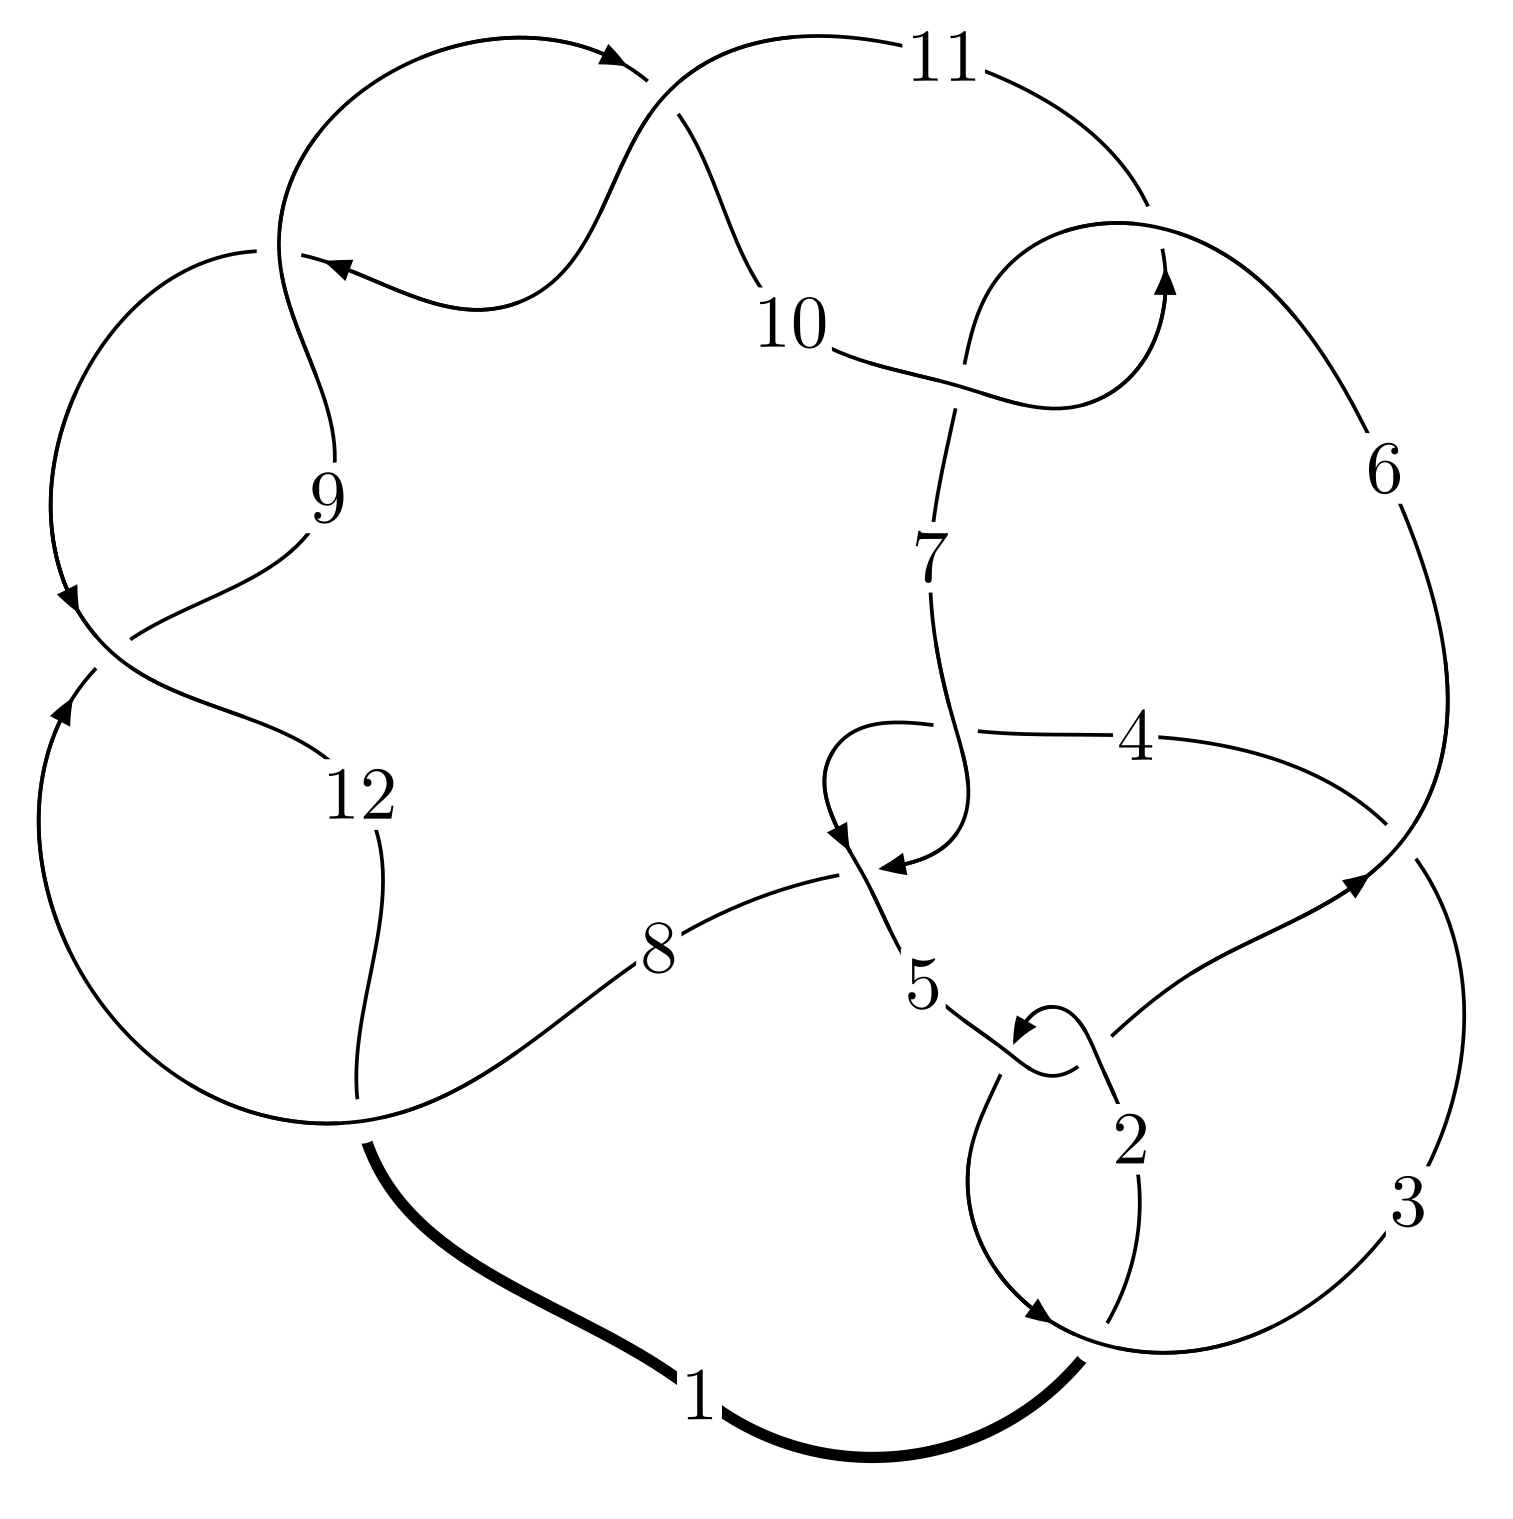
\includegraphics[width=112pt]{../../../GIT/diagram.site/Diagrams/png/2114_12n_0025.png}\\
\ \ \ A knot diagram\footnotemark}&
\allowdisplaybreaks
\textbf{Linearized knot diagam} \\
\cline{2-2}
 &
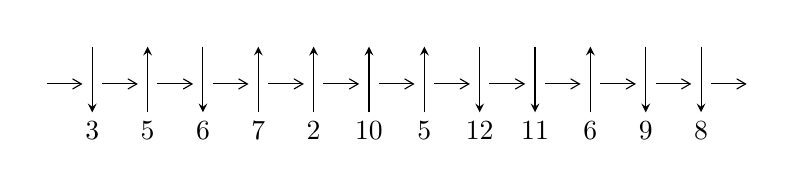
\begin{tikzpicture}[x=20pt, y=17pt]
	% nodes
	\node (C0) at (0, 0) {};
	\node (C1) at (1, 0) {};
	\node (C1U) at (1, +1) {};
	\node (C1D) at (1, -1) {3};

	\node (C2) at (2, 0) {};
	\node (C2U) at (2, +1) {};
	\node (C2D) at (2, -1) {5};

	\node (C3) at (3, 0) {};
	\node (C3U) at (3, +1) {};
	\node (C3D) at (3, -1) {6};

	\node (C4) at (4, 0) {};
	\node (C4U) at (4, +1) {};
	\node (C4D) at (4, -1) {7};

	\node (C5) at (5, 0) {};
	\node (C5U) at (5, +1) {};
	\node (C5D) at (5, -1) {2};

	\node (C6) at (6, 0) {};
	\node (C6U) at (6, +1) {};
	\node (C6D) at (6, -1) {10};

	\node (C7) at (7, 0) {};
	\node (C7U) at (7, +1) {};
	\node (C7D) at (7, -1) {5};

	\node (C8) at (8, 0) {};
	\node (C8U) at (8, +1) {};
	\node (C8D) at (8, -1) {12};

	\node (C9) at (9, 0) {};
	\node (C9U) at (9, +1) {};
	\node (C9D) at (9, -1) {11};

	\node (C10) at (10, 0) {};
	\node (C10U) at (10, +1) {};
	\node (C10D) at (10, -1) {6};

	\node (C11) at (11, 0) {};
	\node (C11U) at (11, +1) {};
	\node (C11D) at (11, -1) {9};

	\node (C12) at (12, 0) {};
	\node (C12U) at (12, +1) {};
	\node (C12D) at (12, -1) {8};
	\node (C13) at (13, 0) {};

	% arrows
	\draw[->,>={angle 60}]
	(C0) edge (C1) (C1) edge (C2) (C2) edge (C3) (C3) edge (C4) (C4) edge (C5) (C5) edge (C6) (C6) edge (C7) (C7) edge (C8) (C8) edge (C9) (C9) edge (C10) (C10) edge (C11) (C11) edge (C12) (C12) edge (C13) ;	\draw[->,>=stealth]
	(C1U) edge (C1D) (C2D) edge (C2U) (C3U) edge (C3D) (C4D) edge (C4U) (C5D) edge (C5U) (C6D) edge (C6U) (C7D) edge (C7U) (C8U) edge (C8D) (C9U) edge (C9D) (C10D) edge (C10U) (C11U) edge (C11D) (C12U) edge (C12D) ;
	\end{tikzpicture} \\
\hhline{~~} \\& 
\textbf{Solving Sequence} \\ \cline{2-2} 
 &
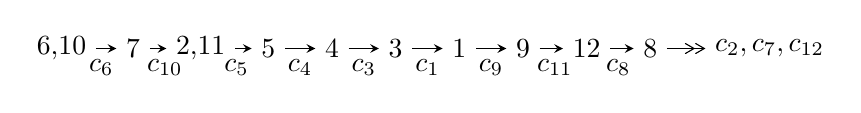
\begin{tikzpicture}[x=23pt, y=7pt]
	% node
	\node (A0) at (-1/8, 0) {6,10};
	\node (A1) at (1, 0) {7};
	\node (A2) at (33/16, 0) {2,11};
	\node (A3) at (25/8, 0) {5};
	\node (A4) at (33/8, 0) {4};
	\node (A5) at (41/8, 0) {3};
	\node (A6) at (49/8, 0) {1};
	\node (A7) at (57/8, 0) {9};
	\node (A8) at (65/8, 0) {12};
	\node (A9) at (73/8, 0) {8};
	\node (C1) at (1/2, -1) {$c_{6}$};
	\node (C2) at (3/2, -1) {$c_{10}$};
	\node (C3) at (21/8, -1) {$c_{5}$};
	\node (C4) at (29/8, -1) {$c_{4}$};
	\node (C5) at (37/8, -1) {$c_{3}$};
	\node (C6) at (45/8, -1) {$c_{1}$};
	\node (C7) at (53/8, -1) {$c_{9}$};
	\node (C8) at (61/8, -1) {$c_{11}$};
	\node (C9) at (69/8, -1) {$c_{8}$};
	\node (A10) at (11, 0) {$c_{2},c_{7},c_{12}$};

	% edge
	\draw[->,>=stealth]	
	(A0) edge (A1) (A1) edge (A2) (A2) edge (A3) (A3) edge (A4) (A4) edge (A5) (A5) edge (A6) (A6) edge (A7) (A7) edge (A8) (A8) edge (A9) ;
	\draw[->>,>={angle 60}]	
	(A9) edge (A10);
\end{tikzpicture} \\ 

\end{tabular} \\

\footnotetext{
The image of knot diagram is generated by the software ``\textbf{Draw programme}" developed by Andrew Bartholomew(\url{http://www.layer8.co.uk/maths/draw/index.htm\#Running-draw}), where we modified some parts for our purpose(\url{https://github.com/CATsTAILs/LinksPainter}).
}\phantom \\ \newline 
\centering \textbf{Ideals for irreducible components\footnotemark of $X_{\text{par}}$} 
 
\begin{align*}
I^u_{1}&=\langle 
u^{11}+2 u^{10}+2 u^9+3 u^7+6 u^6+6 u^5-2 u^4-3 u^3-3 u^2+2 b,\\
\phantom{I^u_{1}}&\phantom{= \langle  }u^{11}+2 u^{10}+u^9-2 u^8+u^7+6 u^6+3 u^5-8 u^4-9 u^3- u^2+2 a+3 u+1,\\
\phantom{I^u_{1}}&\phantom{= \langle  }u^{13}+3 u^{12}+5 u^{11}+4 u^{10}+6 u^9+11 u^8+17 u^7+12 u^6+6 u^5+u^2+u+1\rangle \\
I^u_{2}&=\langle 
u^3 a+2 u^2 a+u^3- a u+2 u^2+8 b-3 a- u-3,\;- u^2 a- u^3+a^2+a u+3 u^2-3 u+2,\;u^4- u^3+u^2+1\rangle \\
\\
\end{align*}
\raggedright * 2 irreducible components of $\dim_{\mathbb{C}}=0$, with total 21 representations.\\
\footnotetext{All coefficients of polynomials are rational numbers. But the coefficients are sometimes approximated in decimal forms when there is not enough margin.}
\newpage
\renewcommand{\arraystretch}{1}
\centering \section*{I. $I^u_{1}= \langle u^{11}+2 u^{10}+\cdots-3 u^2+2 b,\;u^{11}+2 u^{10}+\cdots+2 a+1,\;u^{13}+3 u^{12}+\cdots+u+1 \rangle$}
\flushleft \textbf{(i) Arc colorings}\\
\begin{tabular}{m{7pt} m{180pt} m{7pt} m{180pt} }
\flushright $a_{6}=$&$\begin{pmatrix}1\\0\end{pmatrix}$ \\
\flushright $a_{10}=$&$\begin{pmatrix}0\\u\end{pmatrix}$ \\
\flushright $a_{7}=$&$\begin{pmatrix}1\\- u^2\end{pmatrix}$ \\
\flushright $a_{2}=$&$\begin{pmatrix}-\frac{1}{2} u^{11}- u^{10}+\cdots-\frac{3}{2} u-\frac{1}{2}\\-\frac{1}{2} u^{11}- u^{10}+\cdots+\frac{3}{2} u^3+\frac{3}{2} u^2\end{pmatrix}$ \\
\flushright $a_{11}=$&$\begin{pmatrix}u\\u\end{pmatrix}$ \\
\flushright $a_{5}=$&$\begin{pmatrix}-\frac{1}{2} u^9-\frac{5}{2} u^5-\frac{3}{2} u-\frac{1}{2}\\\frac{1}{2} u^{11}+u^{10}+\cdots+\frac{3}{2} u^3+\frac{3}{2} u^2\end{pmatrix}$ \\
\flushright $a_{4}=$&$\begin{pmatrix}- u^{10}-\frac{3}{2} u^9+\cdots-\frac{3}{2} u-\frac{1}{2}\\u^{12}+\frac{3}{2} u^{11}+\cdots+\frac{3}{2} u^3+\frac{3}{2} u^2\end{pmatrix}$ \\
\flushright $a_{3}=$&$\begin{pmatrix}u^{12}+\frac{3}{2} u^{11}+\cdots-\frac{3}{2} u-\frac{1}{2}\\u^{12}+\frac{3}{2} u^{11}+\cdots+\frac{3}{2} u^3+\frac{3}{2} u^2\end{pmatrix}$ \\
\flushright $a_{1}=$&$\begin{pmatrix}- u^9-3 u^5- u\\- u^9- u^7-3 u^5-2 u^3- u\end{pmatrix}$ \\
\flushright $a_{9}=$&$\begin{pmatrix}u^3\\u^3+u\end{pmatrix}$ \\
\flushright $a_{12}=$&$\begin{pmatrix}u^5+u\\u^5+u^3+u\end{pmatrix}$ \\
\flushright $a_{8}=$&$\begin{pmatrix}u^7+2 u^3\\u^7+u^5+2 u^3+u\end{pmatrix}$\\&\end{tabular}
\flushleft \textbf{(ii) Obstruction class $= -1$}\\~\\
\flushleft \textbf{(iii) Cusp Shapes $= \frac{9}{2} u^{12}+11 u^{11}+15 u^{10}+\frac{11}{2} u^9+\frac{33}{2} u^8+35 u^7+50 u^6+\frac{25}{2} u^5-\frac{11}{2} u^4-\frac{27}{2} u^3+3 u^2+\frac{15}{2} u+\frac{7}{2}$}\\~\\
\newpage\renewcommand{\arraystretch}{1}
\flushleft \textbf{(iv) u-Polynomials at the component}\newline \\
\begin{tabular}{m{50pt}|m{274pt}}
Crossings & \hspace{64pt}u-Polynomials at each crossing \\
\hline $$\begin{aligned}c_{1}\end{aligned}$$&$\begin{aligned}
&u^{13}- u^{12}+\cdots+3 u-1
\end{aligned}$\\
\hline $$\begin{aligned}c_{2},c_{5}\end{aligned}$$&$\begin{aligned}
&u^{13}+5 u^{12}+\cdots-5 u-1
\end{aligned}$\\
\hline $$\begin{aligned}c_{3}\end{aligned}$$&$\begin{aligned}
&u^{13}-5 u^{12}+\cdots-4501 u-833
\end{aligned}$\\
\hline $$\begin{aligned}c_{4},c_{7}\end{aligned}$$&$\begin{aligned}
&u^{13}+u^{12}+\cdots-1152 u-256
\end{aligned}$\\
\hline $$\begin{aligned}c_{6},c_{10}\end{aligned}$$&$\begin{aligned}
&u^{13}-3 u^{12}+5 u^{11}-4 u^{10}+6 u^9-11 u^8+17 u^7-12 u^6+6 u^5- u^2+u-1
\end{aligned}$\\
\hline $$\begin{aligned}c_{8},c_{9},c_{11}\\c_{12}\end{aligned}$$&$\begin{aligned}
&u^{13}+u^{12}+\cdots- u-1
\end{aligned}$\\
\hline
\end{tabular}\\~\\
\newpage\renewcommand{\arraystretch}{1}
\flushleft \textbf{(v) Riley Polynomials at the component}\newline \\
\begin{tabular}{m{50pt}|m{274pt}}
Crossings & \hspace{64pt}Riley Polynomials at each crossing \\
\hline $$\begin{aligned}c_{1}\end{aligned}$$&$\begin{aligned}
&y^{13}+35 y^{12}+\cdots-129 y-1
\end{aligned}$\\
\hline $$\begin{aligned}c_{2},c_{5}\end{aligned}$$&$\begin{aligned}
&y^{13}- y^{12}+\cdots+3 y-1
\end{aligned}$\\
\hline $$\begin{aligned}c_{3}\end{aligned}$$&$\begin{aligned}
&y^{13}+47 y^{12}+\cdots-4829293 y-693889
\end{aligned}$\\
\hline $$\begin{aligned}c_{4},c_{7}\end{aligned}$$&$\begin{aligned}
&y^{13}-45 y^{12}+\cdots-212992 y-65536
\end{aligned}$\\
\hline $$\begin{aligned}c_{6},c_{10}\end{aligned}$$&$\begin{aligned}
&y^{13}+y^{12}+\cdots- y-1
\end{aligned}$\\
\hline $$\begin{aligned}c_{8},c_{9},c_{11}\\c_{12}\end{aligned}$$&$\begin{aligned}
&y^{13}+25 y^{12}+\cdots- y-1
\end{aligned}$\\
\hline
\end{tabular}\\~\\
\newpage\flushleft \textbf{(vi) Complex Volumes and Cusp Shapes}
$$\begin{array}{c|c|c}  
\text{Solutions to }I^u_{1}& \I (\text{vol} + \sqrt{-1}CS) & \text{Cusp shape}\\
 \hline 
\begin{aligned}
u &= -0.440311 + 0.759939 I \\
a &= \phantom{-}0.796729 + 0.648672 I \\
b &= -0.267976 + 0.211150 I\end{aligned}
 & \phantom{-}0.01165 - 1.74285 I & \phantom{-}0.51102 + 3.65273 I \\ \hline\begin{aligned}
u &= -0.440311 - 0.759939 I \\
a &= \phantom{-}0.796729 - 0.648672 I \\
b &= -0.267976 - 0.211150 I\end{aligned}
 & \phantom{-}0.01165 + 1.74285 I & \phantom{-}0.51102 - 3.65273 I \\ \hline\begin{aligned}
u &= -0.748468\phantom{ +0.000000I} \\
a &= \phantom{-}0.262818\phantom{ +0.000000I} \\
b &= \phantom{-}0.939012\phantom{ +0.000000I}\end{aligned}
 & \phantom{-}1.70389\phantom{ +0.000000I} & \phantom{-}6.48230\phantom{ +0.000000I} \\ \hline\begin{aligned}
u &= -0.082679 + 0.714751 I \\
a &= \phantom{-}1.41033 - 2.09260 I \\
b &= \phantom{-}0.247845 - 0.688505 I\end{aligned}
 & -1.32993 - 1.48407 I & -5.25082 + 4.83992 I \\ \hline\begin{aligned}
u &= -0.082679 - 0.714751 I \\
a &= \phantom{-}1.41033 + 2.09260 I \\
b &= \phantom{-}0.247845 + 0.688505 I\end{aligned}
 & -1.32993 + 1.48407 I & -5.25082 - 4.83992 I \\ \hline\begin{aligned}
u &= \phantom{-}0.939578 + 0.989792 I \\
a &= -0.103034 - 0.771838 I \\
b &= -1.151440 - 0.150255 I\end{aligned}
 & \phantom{-}8.78280 + 3.51047 I & \phantom{-}4.53999 - 2.23004 I \\ \hline\begin{aligned}
u &= \phantom{-}0.939578 - 0.989792 I \\
a &= -0.103034 + 0.771838 I \\
b &= -1.151440 + 0.150255 I\end{aligned}
 & \phantom{-}8.78280 - 3.51047 I & \phantom{-}4.53999 + 2.23004 I \\ \hline\begin{aligned}
u &= \phantom{-}0.532801 + 0.327453 I \\
a &= -1.35777 + 1.25278 I \\
b &= \phantom{-}0.616504 + 0.991708 I\end{aligned}
 & \phantom{-}0.55073 + 2.69724 I & \phantom{-}3.82886 - 1.91679 I \\ \hline\begin{aligned}
u &= \phantom{-}0.532801 - 0.327453 I \\
a &= -1.35777 - 1.25278 I \\
b &= \phantom{-}0.616504 - 0.991708 I\end{aligned}
 & \phantom{-}0.55073 - 2.69724 I & \phantom{-}3.82886 + 1.91679 I \\ \hline\begin{aligned}
u &= -0.99353 + 1.07384 I \\
a &= \phantom{-}0.40970 + 1.86567 I \\
b &= -1.14718 + 1.28471 I\end{aligned}
 & -14.0646 - 8.3921 I & \phantom{-}3.62108 + 3.78756 I\\
 \hline 
 \end{array}$$\newpage$$\begin{array}{c|c|c}  
\text{Solutions to }I^u_{1}& \I (\text{vol} + \sqrt{-1}CS) & \text{Cusp shape}\\
 \hline 
\begin{aligned}
u &= -0.99353 - 1.07384 I \\
a &= \phantom{-}0.40970 - 1.86567 I \\
b &= -1.14718 - 1.28471 I\end{aligned}
 & -14.0646 + 8.3921 I & \phantom{-}3.62108 - 3.78756 I \\ \hline\begin{aligned}
u &= -1.08162 + 0.98798 I \\
a &= -0.787365 - 0.595530 I \\
b &= -1.26726 - 1.23564 I\end{aligned}
 & -13.71940 + 0.78911 I & \phantom{-}4.00870 + 0.19018 I \\ \hline\begin{aligned}
u &= -1.08162 - 0.98798 I \\
a &= -0.787365 + 0.595530 I \\
b &= -1.26726 + 1.23564 I\end{aligned}
 & -13.71940 - 0.78911 I & \phantom{-}4.00870 - 0.19018 I\\
 \hline 
 \end{array}$$\newpage\newpage\renewcommand{\arraystretch}{1}
\centering \section*{II. $I^u_{2}= \langle u^3 a+u^3+\cdots-3 a-3,\;- u^2 a- u^3+a^2+a u+3 u^2-3 u+2,\;u^4- u^3+u^2+1 \rangle$}
\flushleft \textbf{(i) Arc colorings}\\
\begin{tabular}{m{7pt} m{180pt} m{7pt} m{180pt} }
\flushright $a_{6}=$&$\begin{pmatrix}1\\0\end{pmatrix}$ \\
\flushright $a_{10}=$&$\begin{pmatrix}0\\u\end{pmatrix}$ \\
\flushright $a_{7}=$&$\begin{pmatrix}1\\- u^2\end{pmatrix}$ \\
\flushright $a_{2}=$&$\begin{pmatrix}a\\-\frac{1}{8} u^3 a-\frac{1}{8} u^3+\cdots+\frac{3}{8} a+\frac{3}{8}\end{pmatrix}$ \\
\flushright $a_{11}=$&$\begin{pmatrix}u\\u\end{pmatrix}$ \\
\flushright $a_{5}=$&$\begin{pmatrix}\frac{1}{8} u^3 a+\frac{1}{8} u^3+\cdots+\frac{5}{8} a-\frac{3}{8}\\-\frac{1}{8} u^3 a-\frac{1}{8} u^3+\cdots+\frac{3}{8} a-\frac{5}{8}\end{pmatrix}$ \\
\flushright $a_{4}=$&$\begin{pmatrix}\frac{1}{8} u^3 a+\frac{1}{8} u^3+\cdots+\frac{5}{8} a-\frac{3}{8}\\-\frac{1}{8} u^3 a-\frac{1}{8} u^3+\cdots+\frac{3}{8} a-\frac{5}{8}\end{pmatrix}$ \\
\flushright $a_{3}=$&$\begin{pmatrix}- u^2+a+u-1\\-\frac{1}{8} u^3 a-\frac{1}{8} u^3+\cdots+\frac{3}{8} a-\frac{5}{8}\end{pmatrix}$ \\
\flushright $a_{1}=$&$\begin{pmatrix}-1\\0\end{pmatrix}$ \\
\flushright $a_{9}=$&$\begin{pmatrix}u^3\\u^3+u\end{pmatrix}$ \\
\flushright $a_{12}=$&$\begin{pmatrix}- u^2-1\\u^3- u^2-1\end{pmatrix}$ \\
\flushright $a_{8}=$&$\begin{pmatrix}1\\- u^2\end{pmatrix}$\\&\end{tabular}
\flushleft \textbf{(ii) Obstruction class $= 1$}\\~\\
\flushleft \textbf{(iii) Cusp Shapes $= -\frac{1}{2} u^3 a+2 u^2 a+\frac{1}{2} u^3-\frac{3}{2} a u-3 u^2-\frac{1}{2} a+\frac{5}{2} u+\frac{1}{2}$}\\~\\
\newpage\renewcommand{\arraystretch}{1}
\flushleft \textbf{(iv) u-Polynomials at the component}\newline \\
\begin{tabular}{m{50pt}|m{274pt}}
Crossings & \hspace{64pt}u-Polynomials at each crossing \\
\hline $$\begin{aligned}c_{1},c_{3},c_{5}\end{aligned}$$&$\begin{aligned}
&(u^2- u+1)^4
\end{aligned}$\\
\hline $$\begin{aligned}c_{2}\end{aligned}$$&$\begin{aligned}
&(u^2+u+1)^4
\end{aligned}$\\
\hline $$\begin{aligned}c_{4},c_{7}\end{aligned}$$&$\begin{aligned}
&u^8
\end{aligned}$\\
\hline $$\begin{aligned}c_{6}\end{aligned}$$&$\begin{aligned}
&(u^4- u^3+u^2+1)^2
\end{aligned}$\\
\hline $$\begin{aligned}c_{8},c_{9}\end{aligned}$$&$\begin{aligned}
&(u^4- u^3+3 u^2-2 u+1)^2
\end{aligned}$\\
\hline $$\begin{aligned}c_{10}\end{aligned}$$&$\begin{aligned}
&(u^4+u^3+u^2+1)^2
\end{aligned}$\\
\hline $$\begin{aligned}c_{11},c_{12}\end{aligned}$$&$\begin{aligned}
&(u^4+u^3+3 u^2+2 u+1)^2
\end{aligned}$\\
\hline
\end{tabular}\\~\\
\newpage\renewcommand{\arraystretch}{1}
\flushleft \textbf{(v) Riley Polynomials at the component}\newline \\
\begin{tabular}{m{50pt}|m{274pt}}
Crossings & \hspace{64pt}Riley Polynomials at each crossing \\
\hline $$\begin{aligned}c_{1},c_{2},c_{3}\\c_{5}\end{aligned}$$&$\begin{aligned}
&(y^2+y+1)^4
\end{aligned}$\\
\hline $$\begin{aligned}c_{4},c_{7}\end{aligned}$$&$\begin{aligned}
&y^8
\end{aligned}$\\
\hline $$\begin{aligned}c_{6},c_{10}\end{aligned}$$&$\begin{aligned}
&(y^4+y^3+3 y^2+2 y+1)^2
\end{aligned}$\\
\hline $$\begin{aligned}c_{8},c_{9},c_{11}\\c_{12}\end{aligned}$$&$\begin{aligned}
&(y^4+5 y^3+7 y^2+2 y+1)^2
\end{aligned}$\\
\hline
\end{tabular}\\~\\
\newpage\flushleft \textbf{(vi) Complex Volumes and Cusp Shapes}
$$\begin{array}{c|c|c}  
\text{Solutions to }I^u_{2}& \I (\text{vol} + \sqrt{-1}CS) & \text{Cusp shape}\\
 \hline 
\begin{aligned}
u &= -0.351808 + 0.720342 I \\
a &= \phantom{-}1.04112 + 1.08095 I \\
b &= \phantom{-}0.500000 + 0.866025 I\end{aligned}
 & -0.211005 + 0.614778 I & \phantom{-}2.20786 + 0.04655 I \\ \hline\begin{aligned}
u &= -0.351808 + 0.720342 I \\
a &= -1.08443 - 2.30813 I \\
b &= \phantom{-}0.500000 - 0.866025 I\end{aligned}
 & -0.21101 - 3.44499 I & -2.55284 + 7.82341 I \\ \hline\begin{aligned}
u &= -0.351808 - 0.720342 I \\
a &= \phantom{-}1.04112 - 1.08095 I \\
b &= \phantom{-}0.500000 - 0.866025 I\end{aligned}
 & -0.211005 - 0.614778 I & \phantom{-}2.20786 - 0.04655 I \\ \hline\begin{aligned}
u &= -0.351808 - 0.720342 I \\
a &= -1.08443 + 2.30813 I \\
b &= \phantom{-}0.500000 + 0.866025 I\end{aligned}
 & -0.21101 + 3.44499 I & -2.55284 - 7.82341 I \\ \hline\begin{aligned}
u &= \phantom{-}0.851808 + 0.911292 I \\
a &= \phantom{-}0.076953 - 0.582938 I \\
b &= \phantom{-}0.500000 - 0.866025 I\end{aligned}
 & \phantom{-}6.79074 + 1.13408 I & \phantom{-}2.75261 - 0.95911 I \\ \hline\begin{aligned}
u &= \phantom{-}0.851808 + 0.911292 I \\
a &= -1.03364 + 1.22414 I \\
b &= \phantom{-}0.500000 + 0.866025 I\end{aligned}
 & \phantom{-}6.79074 + 5.19385 I & \phantom{-}2.09237 - 4.44058 I \\ \hline\begin{aligned}
u &= \phantom{-}0.851808 - 0.911292 I \\
a &= \phantom{-}0.076953 + 0.582938 I \\
b &= \phantom{-}0.500000 + 0.866025 I\end{aligned}
 & \phantom{-}6.79074 - 1.13408 I & \phantom{-}2.75261 + 0.95911 I \\ \hline\begin{aligned}
u &= \phantom{-}0.851808 - 0.911292 I \\
a &= -1.03364 - 1.22414 I \\
b &= \phantom{-}0.500000 - 0.866025 I\end{aligned}
 & \phantom{-}6.79074 - 5.19385 I & \phantom{-}2.09237 + 4.44058 I\\
 \hline 
 \end{array}$$\newpage
\newpage\renewcommand{\arraystretch}{1}
\centering \section*{ III. u-Polynomials}
\begin{tabular}{m{50pt}|m{274pt}}
Crossings & \hspace{64pt}u-Polynomials at each crossing \\
\hline $$\begin{aligned}c_{1}\end{aligned}$$&$\begin{aligned}
&((u^2- u+1)^4)(u^{13}- u^{12}+\cdots+3 u-1)
\end{aligned}$\\
\hline $$\begin{aligned}c_{2}\end{aligned}$$&$\begin{aligned}
&((u^2+u+1)^4)(u^{13}+5 u^{12}+\cdots-5 u-1)
\end{aligned}$\\
\hline $$\begin{aligned}c_{3}\end{aligned}$$&$\begin{aligned}
&((u^2- u+1)^4)(u^{13}-5 u^{12}+\cdots-4501 u-833)
\end{aligned}$\\
\hline $$\begin{aligned}c_{4},c_{7}\end{aligned}$$&$\begin{aligned}
&u^8(u^{13}+u^{12}+\cdots-1152 u-256)
\end{aligned}$\\
\hline $$\begin{aligned}c_{5}\end{aligned}$$&$\begin{aligned}
&((u^2- u+1)^4)(u^{13}+5 u^{12}+\cdots-5 u-1)
\end{aligned}$\\
\hline $$\begin{aligned}c_{6}\end{aligned}$$&$\begin{aligned}
&(u^4- u^3+u^2+1)^2\\
&\cdot(u^{13}-3 u^{12}+5 u^{11}-4 u^{10}+6 u^9-11 u^8+17 u^7-12 u^6+6 u^5- u^2+u-1)
\end{aligned}$\\
\hline $$\begin{aligned}c_{8},c_{9}\end{aligned}$$&$\begin{aligned}
&((u^4- u^3+3 u^2-2 u+1)^2)(u^{13}+u^{12}+\cdots- u-1)
\end{aligned}$\\
\hline $$\begin{aligned}c_{10}\end{aligned}$$&$\begin{aligned}
&(u^4+u^3+u^2+1)^2\\
&\cdot(u^{13}-3 u^{12}+5 u^{11}-4 u^{10}+6 u^9-11 u^8+17 u^7-12 u^6+6 u^5- u^2+u-1)
\end{aligned}$\\
\hline $$\begin{aligned}c_{11},c_{12}\end{aligned}$$&$\begin{aligned}
&((u^4+u^3+3 u^2+2 u+1)^2)(u^{13}+u^{12}+\cdots- u-1)
\end{aligned}$\\
\hline
\end{tabular}\newpage\renewcommand{\arraystretch}{1}
\centering \section*{ IV. Riley Polynomials}
\begin{tabular}{m{50pt}|m{274pt}}
Crossings & \hspace{64pt}Riley Polynomials at each crossing \\
\hline $$\begin{aligned}c_{1}\end{aligned}$$&$\begin{aligned}
&((y^2+y+1)^4)(y^{13}+35 y^{12}+\cdots-129 y-1)
\end{aligned}$\\
\hline $$\begin{aligned}c_{2},c_{5}\end{aligned}$$&$\begin{aligned}
&((y^2+y+1)^4)(y^{13}- y^{12}+\cdots+3 y-1)
\end{aligned}$\\
\hline $$\begin{aligned}c_{3}\end{aligned}$$&$\begin{aligned}
&((y^2+y+1)^4)(y^{13}+47 y^{12}+\cdots-4829293 y-693889)
\end{aligned}$\\
\hline $$\begin{aligned}c_{4},c_{7}\end{aligned}$$&$\begin{aligned}
&y^8(y^{13}-45 y^{12}+\cdots-212992 y-65536)
\end{aligned}$\\
\hline $$\begin{aligned}c_{6},c_{10}\end{aligned}$$&$\begin{aligned}
&((y^4+y^3+3 y^2+2 y+1)^2)(y^{13}+y^{12}+\cdots- y-1)
\end{aligned}$\\
\hline $$\begin{aligned}c_{8},c_{9},c_{11}\\c_{12}\end{aligned}$$&$\begin{aligned}
&((y^4+5 y^3+7 y^2+2 y+1)^2)(y^{13}+25 y^{12}+\cdots- y-1)
\end{aligned}$\\
\hline
\end{tabular}
\vskip 2pc
\end{document}